\chapter{LBR-Stack: ROS 2 and Python Integration of KUKA FRI for Med and
IIWA Robots}
\label{app:lbr_stack}
\minitoc

\paragraph{Disclaimer} This \appref{app:lbr_stack} is an \textit{in extenso} reproduction of \cite{huber2023lbr}. Only \secref{c2:sec:introduction} was altered to highlight additional context within the scope of this thesis.

\newpage

\begin{figure}
\centering
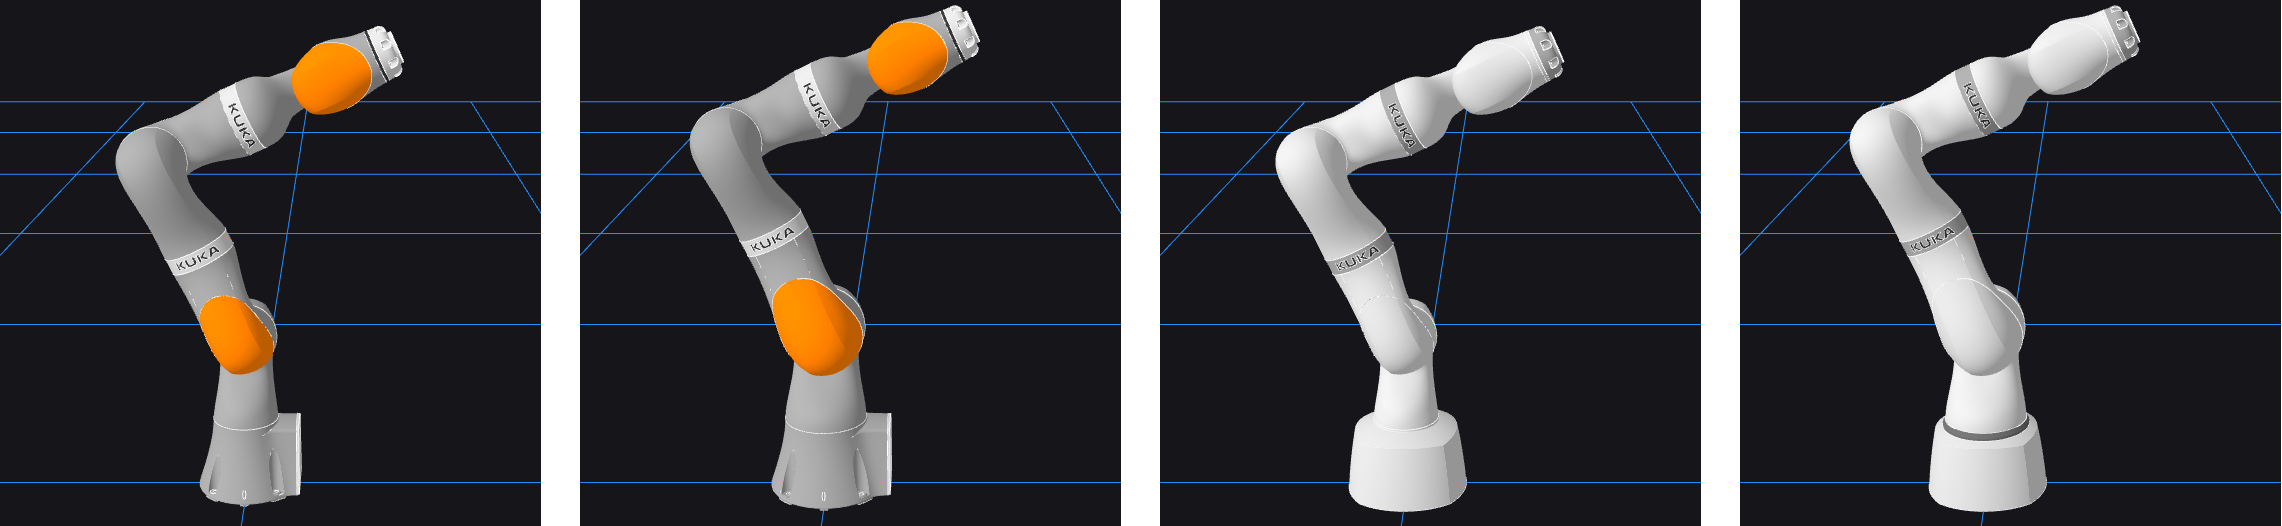
\includegraphics[width=\textwidth]{appendix_1/img/joss_figure.png}
\caption[Supported robots in the LBR-Stack. From left to right: KUKA LBR
IIWA7, IIWA14, Med7, Med14. Visualizations made using Foxglove
.]{Supported robots in the LBR-Stack. From left to right: KUKA LBR
IIWA7, IIWA14, Med7, Med14. Visualizations made using Foxglove
\footnotemark{}.}
\end{figure}
\footnotetext{Foxglove: \url{https://foxglove.dev/ros}.}

\hypertarget{summary}{%
\section{Summary}\label{summary}}
The \texttt{LBR-Stack} is a collection of packages that simplify the
usage and extend the capabilities of KUKA's Fast Robot Interface (FRI)
\cite{ref-fri}. It is designed
for mission critical hard real-time applications. Supported are the
\texttt{KUKA\ LBR\ Med7/14} and \texttt{KUKA\ LBR\ IIWA7/14} robots in
the Gazebo simulation \cite{ref-gazebo} and for communication with real hardware. A demo video can be
found
\href{https://www.linkedin.com/posts/mhubii_robotics-opensource-ros2-activity-7009974676017848320-S3U5/?utm_source=share\&utm_medium=member_desktop}{here}.
An overview of the software architecture is shown in Figure
\ref{fig:fri}.

At the \texttt{LBR-Stack}'s core are two packages:

\begin{itemize}
\item
  \textbf{fri}: Integration of KUKA's original FRI client library into
  CMake.
\item
  \textbf{fri\_vendor}: Vendor library that integrates the \textbf{fri}
  into the ROS 2 build sytem.
\end{itemize}

All other packages are built on top. These include Python bindings and
packages for integration into the Robot Operating System (ROS) and ROS
2:

\begin{itemize}
\item
  \textbf{pyFRI}: Python bindings for the \textbf{fri}.
\item
  \textbf{lbr\_fri\_ros2\_stack}: ROS 1/2 integration of the
  \texttt{KUKA\ LBR}s through the \textbf{fri\_vendor}.
\end{itemize}

For brevity, and due to the architectural advantages over ROS
\cite{ref-ros2}, only ROS 2 is
considered in the following. The \textbf{lbr\_fri\_ros2\_stack}
comprises the following packages:

\begin{itemize}
\item
  \textbf{lbr\_bringup}: Python library for launching the different
  components.
\item
  \textbf{lbr\_description}: Description files for the \texttt{Med7/14}
  and \texttt{IIWA7/14} robots.
\item
  \textbf{lbr\_demos}: Demonstrations for simulation and the real
  robots.
\item
  \textbf{lbr\_fri\_msgs}: Interface Definition Language (IDL)
  equivalent of FRI protocol buffers.
\item
  \textbf{lbr\_fri\_ros2}: FRI ROS 2 interface through
  \texttt{realtime\_tools} \cite{ref-ros_control}.
\item
  \textbf{lbr\_ros2\_control}: Interface and controllers for
  \texttt{ros2\_control} \cite{ref-ros2_control}.
\item
  \textbf{lbr\_moveit\_config}: MoveIt 2 configurations
  \cite{ref-moveit}.
\end{itemize}

\begin{figure}
\centering
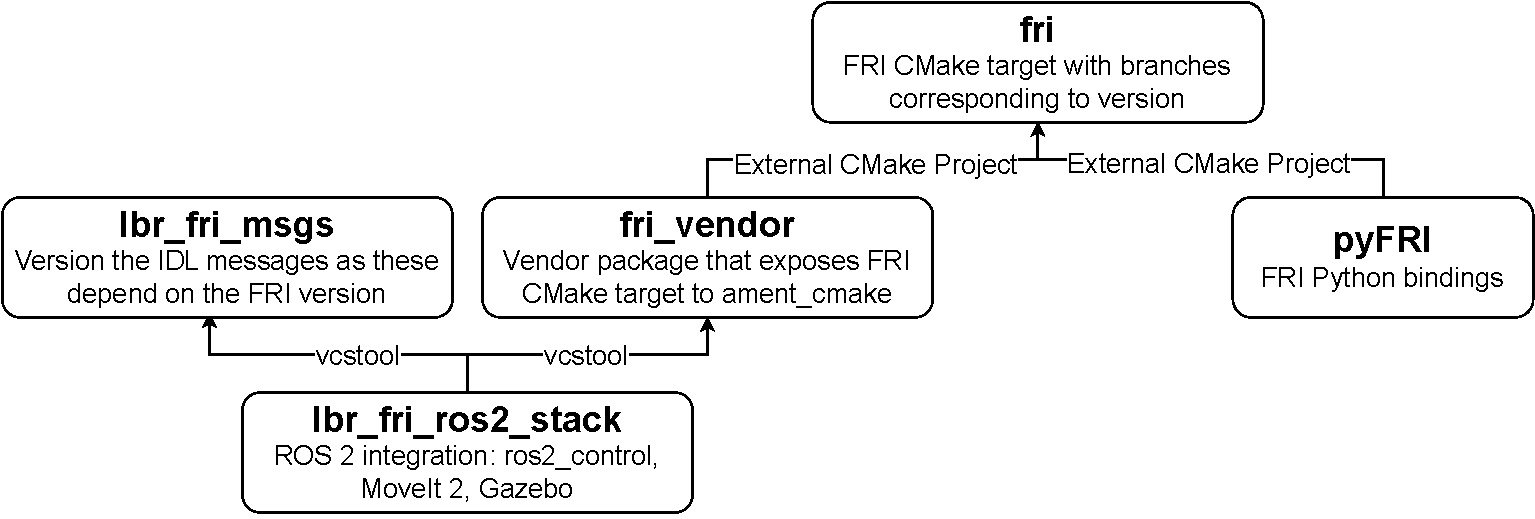
\includegraphics[width=\textwidth]{appendix_1/img/fri_dependency_architecture.pdf}
\caption[An overview of the overall software architecture. There exists
a single source for KUKA's FRI. This design facilitates that downstream
packages, i.e.~the Python bindings and the ROS 2 package, can easily
support multiple FRI versions. The ROS 2 side utilizes
vcstool.\label{fig:fri}]{An overview of the overall software
architecture. There exists a single source for KUKA's FRI. This design
facilitates that downstream packages, i.e.~the Python bindings and the
ROS 2 package, can easily support multiple FRI versions. The ROS 2 side
utilizes vcstool\footnotemark{}.\label{fig:fri}}
\end{figure}
\footnotetext{vcstool: \url{https://github.com/dirk-thomas/vcstool}.}

\hypertarget{statement-of-need}{%
\section{Statement of need}\label{statement-of-need}}

An overview of existing work that interfaces the KUKA LBRs from an
external computer is given in Table 1. We broadly classify these works
into custom communication solutions
\cite{ref-iiwa_stack,ref-kuka_sunrise_toolbox,ref-libiiwa} and
communication solutions through KUKA's FRI UDP channel 
\cite{ref-iiwa_ros2,ref-iiwa_ros}. The
former can offer greater flexibility while the latter offer a well
defined interface and direct software support from KUKA. Contrary to the
custom communication solutions, the FRI solutions additionally enable
hard real-time communication, that is beneficial for mission critical
development. Stemming from translational medical research, this work
therefore focuses on the FRI.

Limitations with the current FRI solutions are:

\begin{enumerate}
\def\labelenumi{\arabic{enumi}.}
\item
  Only support \texttt{IIWA7/14} robots, not \texttt{Med7/14}.
\item
  Don't provide Python bindings.
\item
  Maintainability:

  \begin{itemize}
  \item
    Modified client source code
    \href{https://github.com/epfl-lasa/iiwa_ros}{iiwa\_ros}.
  \item
    FRI client library tangled into source code
    \href{https://github.com/ICube-Robotics/iiwa_ros2}{iiwa\_ros2}.
  \end{itemize}
\item
  Partial support of FRI functionality. Both,
  \href{https://github.com/epfl-lasa/iiwa_ros}{iiwa\_ros} and
  \href{https://github.com/ICube-Robotics/iiwa_ros2}{iiwa\_ros2},
  exclusively aim at providing implementations of the ROS 1/2 hardware
  abstraction layer. This does not support:

  \begin{itemize}
  \item
    FRI's cartesian impedance control mode.
  \item
    FRI's cartesian control mode (FRI version 2 and above).
  \end{itemize}
\end{enumerate}

The first original contribution of this work is to add support for the
\texttt{KUKA\ LBR\ Med7/14} robots, which, to the best author's
knowledge, does not exist in any other work. The second novel
contribution of this work is to provide Python bindings. This work
solves the maintainability by outsourcing the FRI into the separate
\textbf{fri} and \textbf{fri\_vendor} packages, which leaves the FRI's
source code untouched and simply provides build support. 4. is solved by
defining an IDL message to KUKA's \texttt{nanopb} command and state
protocol buffers in \textbf{lbr\_fri\_msgs}. These messages can then be
interfaced from ROS 1/2 topics or from the ROS 1/2 hardware abstraction
layer.

\begin{landscape}
\begin{table}
\centering
\caption{Overview of existing frameworks for interfacing the KUKA LBRs.
A bullet point indicates support for the respective feature.}
\centering
\resizebox{0.7\paperheight}{!}{
\begin{tabular}{llllllllllll}
\hline
Framework                                                                      & IIWA      & Med       & ROS       & ROS 2     & Hard Real-time & FRI       & pyFRI     & Position Control & Impedance Control & Cartesian Impedance Control & Hardware Interface \\ \hline
$\href{https://github.com/lbr-stack}{\text{lbr-stack}}$                        & $\bullet$ & $\bullet$ & $\bullet$ & $\bullet$ & $\bullet$      & $\bullet$ & $\bullet$ & $\bullet$        & $\bullet$         & $\bullet$                   & $\bullet$          \\
$\href{https://github.com/epfl-lasa/iiwa_ros}{\text{iiwa\_ros}}$               & $\bullet$ &           & $\bullet$ &           & $\bullet$      & $\bullet$ &           & $\bullet$        & $\bullet$         &                             & $\bullet$          \\
$\href{https://github.com/ICube-Robotics/iiwa_ros2}{\text{iiwa\_ros2}}$        & $\bullet$ &           &           & $\bullet$ & $\bullet$      & $\bullet$ &           & $\bullet$        & $\bullet$         &                             & $\bullet$          \\
$\href{https://github.com/IFL-CAMP/iiwa_stack}{\text{iiwa-stack}}$             & $\bullet$ &           & $\bullet$ &           &                &           &           & $\bullet$        & $\bullet$         & $\bullet$                   &                    \\
$\href{https://github.com/Toni-SM/libiiwa}{\text{libiiwa}}$                    & $\bullet$ &           & $\bullet$ & $\bullet$ &                &           &           & $\bullet$        & $\bullet$         & $\bullet$                   &                    \\
$\href{https://github.com/Modi1987/KST-Kuka-Sunrise-Toolbox}{\text{KST-KUKA}}$ & $\bullet$ &           &           &           &                &           &           & $\bullet$        & $\bullet$         & $\bullet$                   &                    \\ \hline
\end{tabular}
}
\end{table}
\end{landscape}

\hypertarget{acknowledgement}{%
\section{Acknowledgement}\label{acknowledgement}}

We want to acknowledge the work in
\cite{ref-iiwa_stack}, as
their MoveIt configurations were utilized in a first iteration of this
project.
